\documentclass{report}

\usepackage[T1]{fontenc}
\usepackage[utf8]{inputenc}
\usepackage[brazilian]{babel}
\usepackage{graphicx}
\usepackage[export]{adjustbox}[2011/08/13]
\usepackage{float}
\usepackage[pdftex]{hyperref}
\usepackage{epstopdf}
\usepackage{etoolbox}
\usepackage{amsmath}
\usepackage{amsfonts}
\usepackage{amssymb}
\usepackage{caption}
\usepackage{subcaption}
\usepackage{setspace}
\usepackage{tikz}
\usepackage{listings}
\usepackage{xcolor} 

\bibliographystyle{eric}
\patchcmd{\thebibliography}{\section*}{\section}{}{}


\newcommand{\R}{\ensuremath{\mathbb{R}}}
\newcommand{\Prob}{\ensuremath{\mathbb{P}}}
\newcommand{\K}{\ensuremath{\mathbb{K}}}
\newcommand{\U}{\ensuremath{\mathbb{U}}}
\newcommand{\N}{\ensuremath{\mathbb{N}}}
\newcommand{\Lg}{\ensuremath{\mathbb{L}}}
\newcommand{\T}{\ensuremath{\rm Tr}}
\newcommand{\sg}{{\sigma(x_k)}}

\newcommand{\G}{\ensuremath{\mathcal{G}}}
\newcommand{\F}{\ensuremath{\mathcal{F}}}
\newcommand{\C}{\ensuremath{\mathcal{C}}}
\newcommand{\E}{\ensuremath{\mathcal{E}}}
\newcommand{\Hn}{\ensuremath{\mathcal{H}}}
\newcommand{\Hoo}{\ensuremath{\mathcal{H}_\infty}}
\newcommand{\Hop}{\ensuremath{\mathcal{H}_{op}}}
% --------------------------------------------------
\newtheorem{theo}{Teorema}
\newtheorem{exa}{Exemplo}
\newtheorem{lemm}{Lema}
\newtheorem{coro}{Corolário}
\newtheorem{defn}{Definição}[section]

\begin{document}

\begin{titlepage}
\begin{center}

\newcommand{\HRule}{\rule{\linewidth}{0.5mm}}
% Upper part of the page. The '~' is needed because \\
% only works if a paragraph has started.

\includegraphics[width=0.15\textwidth]{logoUnicamp}~\\[1cm]

\textsc{\LARGE Universidade Estadual de Campinas}\\[1.5cm]

\textsc{\Large Faculdade de Engenharia Mecânica}\\[0.5cm]

% Title
\HRule \\[0.4cm]
{ \huge \bfseries ES664 - Laboratório de Eletrônica para Automação Industrial\\ \vspace{1cm} Relatório - Experimento 4\\
\Large{Acionamento de motor DC} \\[0.4cm] }

\HRule \\[1.5cm]

% Author and supervisor
\begin{minipage}{0.6\textwidth}
\begin{flushleft} \large
\emph{Nome:}\\
Daniel Dello Russo Oliveira\\Marcelli Tiemi Kian
\end{flushleft}
\end{minipage}
\begin{minipage}{0.2\textwidth}
\begin{flushright} \large
\emph{RA}\\ 101918\\117892
\end{flushright}
\end{minipage}

\vfill

% Bottom of the page
{\large \today}

\end{center}
\end{titlepage}


\onehalfspacing
\section{Objetivos}
Este experimento tem como objetivo a familiarização com os equipamentos e instrumentos do laboratório, bem como o estudo de retificadores não controlados para fontes monofásicas e trifásicas.

\section{Materiais e equipamentos}
Foram disponibilizados para o experimento uma fonte trifásica de $V_{LL}=330\ V$, duas lâmpadas de $60\ W$/$220\ V$, kit didático contendo cartão de fusíveis e cartão de diodos, cabos, osciloscópio e multímetro digital.

\section{Retificador monofásico}
Montamos o retificador de onda completa não controlado para fonte monofásica conforme proposto no roteiro do experimento\cite{bb:rexp1}. É importante ressaltar a utilização do fusível de proteção entre a fonte e o restante do circuito, para que eventuais problemas na rede elétrica ou na construção do circuito afetem com severidade os equipamentos.

Tomando os devidos cuidados, utilizamos um canal do osciloscópio para verificar a tensão da fonte monofásica, ou seja, a tensão entre uma fase e o neutro. Obtivemos como resultado a tensão mostrada na figura \ref{fig:mono_s}, com valor de pico $V_{AN}=190\ V$. Este valor é condizente com a fonte trifásica de $V_{LL}=330\ V$.

\begin{figure}[H]
	\centering
	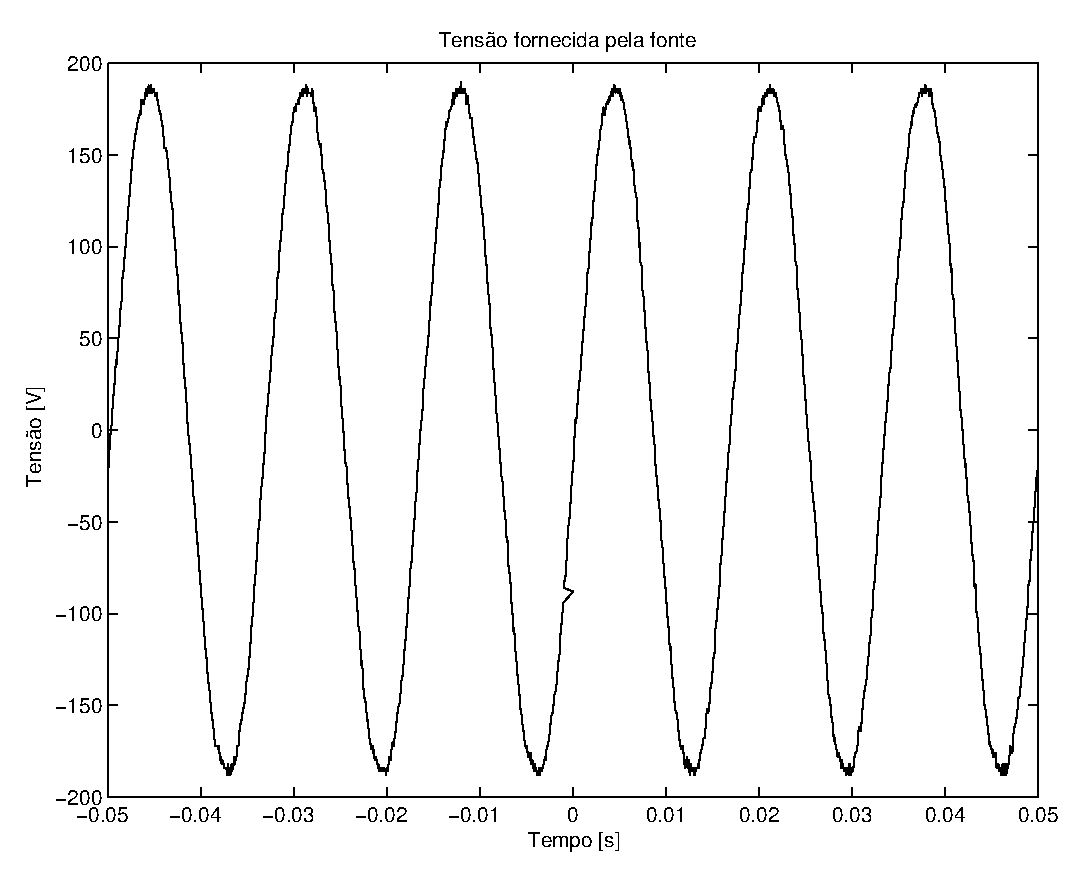
\includegraphics[width=\linewidth]{dados/monofasico/mono_s}
	\caption{Tensão medida na fonte monofásica}
	\label{fig:mono_s}
\end{figure}

Desligamos o circuito e posicionamos os canais do osciloscópio para capturar dados das tensões nos diodos D3 e D6. Religando a chave, obtivemos as leituras apresentadas nas figuras \ref{fig:mono_d3} e \ref{fig:mono_d6}, onde as tensões de pico foram $V_{D3}=190\ V$ e $V_{D6}=188\ V$. Utilizando a função matemática disponível no osciloscópio, fizemos a diferença de tensão entre os dois canais, obtendo assim a leitura da tensão sobre a carga $v_o$ mostrada na figura \ref{fig:mono_r}.

\begin{figure}[H]
	\centering
	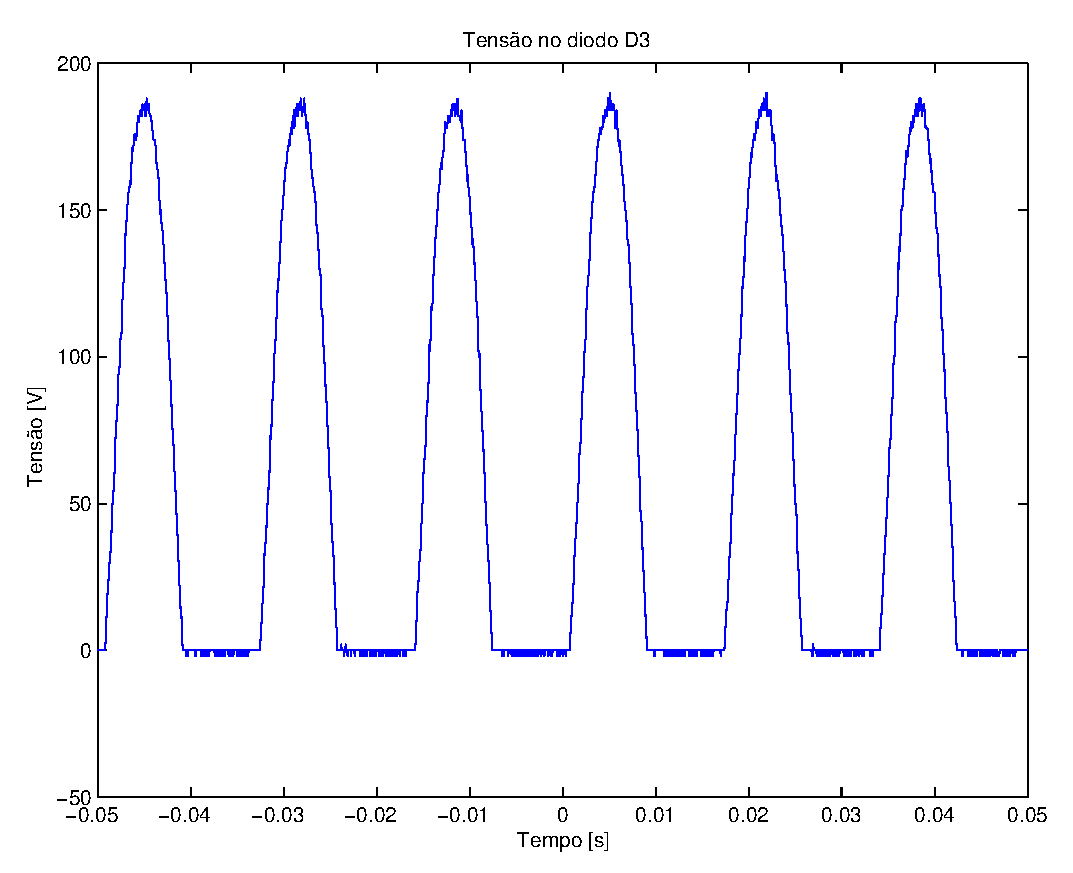
\includegraphics[width=\linewidth]{dados/monofasico/mono_d3}
	\caption{Tensão medida no diodo D3}
	\label{fig:mono_d3}
\end{figure}

\begin{figure}[H]
	\centering
	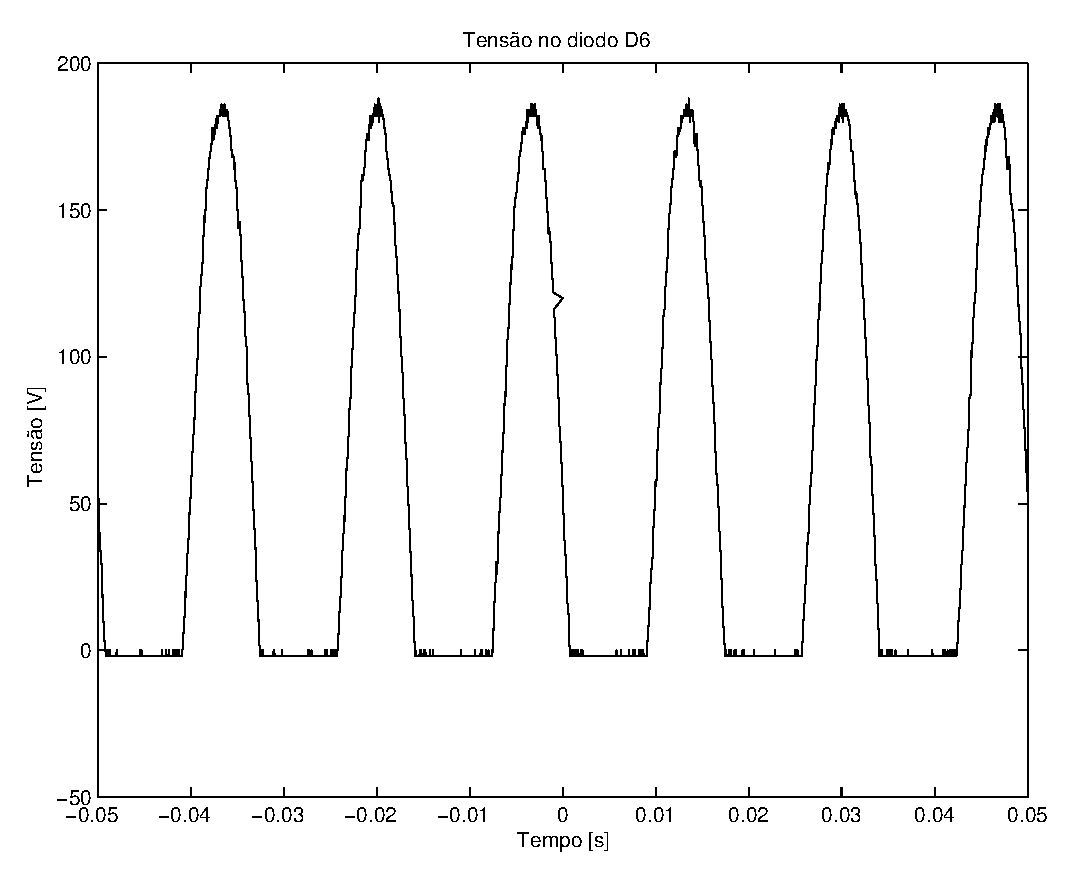
\includegraphics[width=\linewidth]{dados/monofasico/mono_d6}
	\caption{Tensão medida no diodo D6}
	\label{fig:mono_d6}
\end{figure}

\begin{figure}[H]
	\centering
	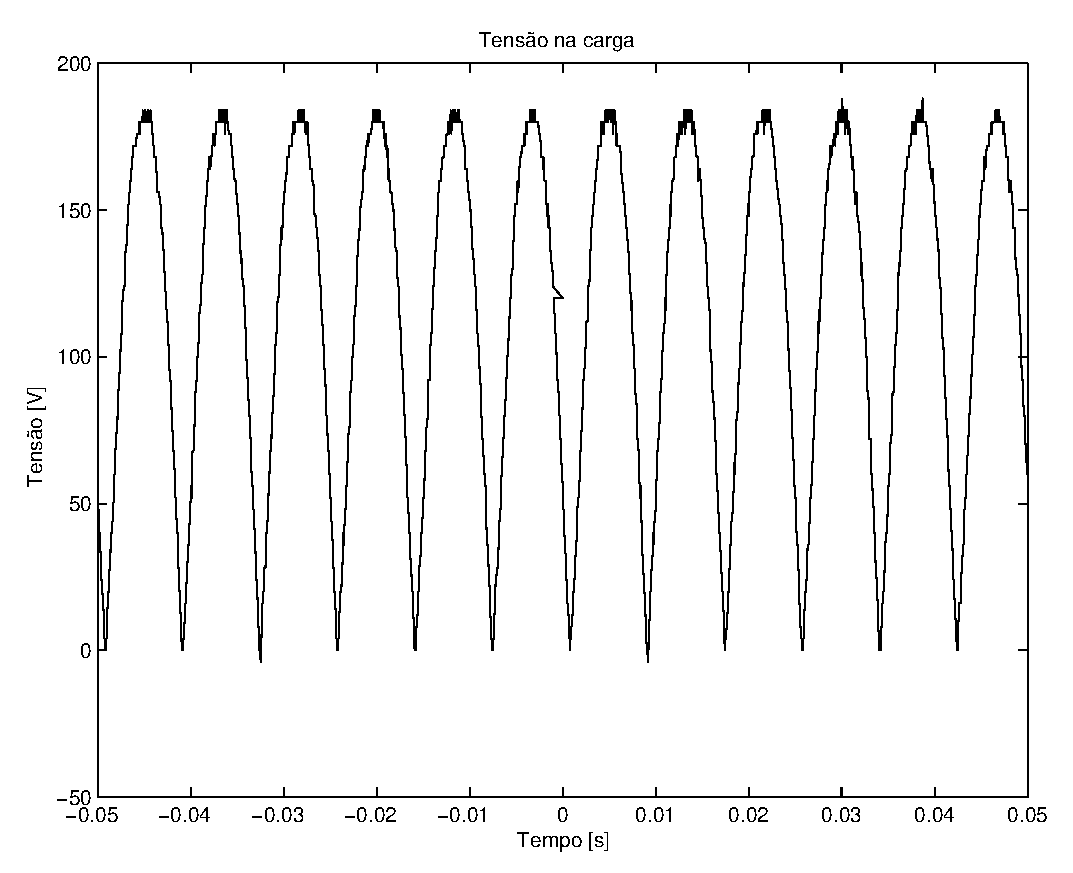
\includegraphics[width=\linewidth]{dados/monofasico/mono_r}
	\caption{Tensão medida na lâmpada}
	\label{fig:mono_r}
\end{figure}

Ainda com auxílio do osciloscópio, verificamos os valores médio e RMS para a tensão na carga:
\begin{equation}
\overline{v_o} = 116\ V
\end{equation}
\begin{equation}
v_{o_{rms}} = 130\ V
\end{equation}

Desligamos o circuito e medimos com auxílio do multímetro a resistência da lâmpada, obtendo como resultado $R_1=70.1\ \Omega$.

%TODO: fazer cálculos teóricos para comparar (monofásico)
Podemos calcular a tensão média teórica sobre a carga através da equação \ref{eq:mmean}
\begin{equation}
\overline{Vr} = \frac{1}{\pi} \int_{0}^{\pi}{Vs sin(\theta)d\theta} = \frac{2 Vs}{\pi}
\label{eq:mmean}
\end{equation}
Para calcular o valor efetivo da tensão sobre a carga utilizamos a equação \ref{eq:mrms}.
\begin{equation}
Vr_{rms} = \sqrt{\frac{1}{\pi} \int_{0}^{\pi}{(Vs sin(\theta))^2 d\theta}} = \frac{Vs}{\sqrt{2}}
\label{eq:mrms}
\end{equation}
Substituindo a tensão da fonte ($Vs\ =\ 190\ V$), encontramos as tensões esperadas:
\begin{equation}
\overline{Vr} = 120.9575\ V
\end{equation}
\begin{equation}
Vr_{rms} =  134,3503\ V
\end{equation}
Conforme podemos ver os valores medidos e esperados diferem levemente, isso acontece devido a uma série de fatores, entre eles a queda de tensão nos diodos, as variações na tensão da fonte e as imprecisões da medida.


Estimamos a queda de tensão nos diodos de duas maneiras: Uma pela análise direta das curvas dos diodos, cuja a tensão quando estão conduzindo assume um valor de aproximadamente $2 V$. A outra maneira consistiu em encontrar a diferença entre o valor absoluto da tensão na fonte e a tensão, para isso tivemos que ajustar os dados medidos para remover a defasagem entre as medidas e filtrar os sinais para remover o ruído da medida, obtendo as curvas das figuras \ref{fig:abs} e \ref{fig:diff}.

\begin{figure}[H]
	\centering
	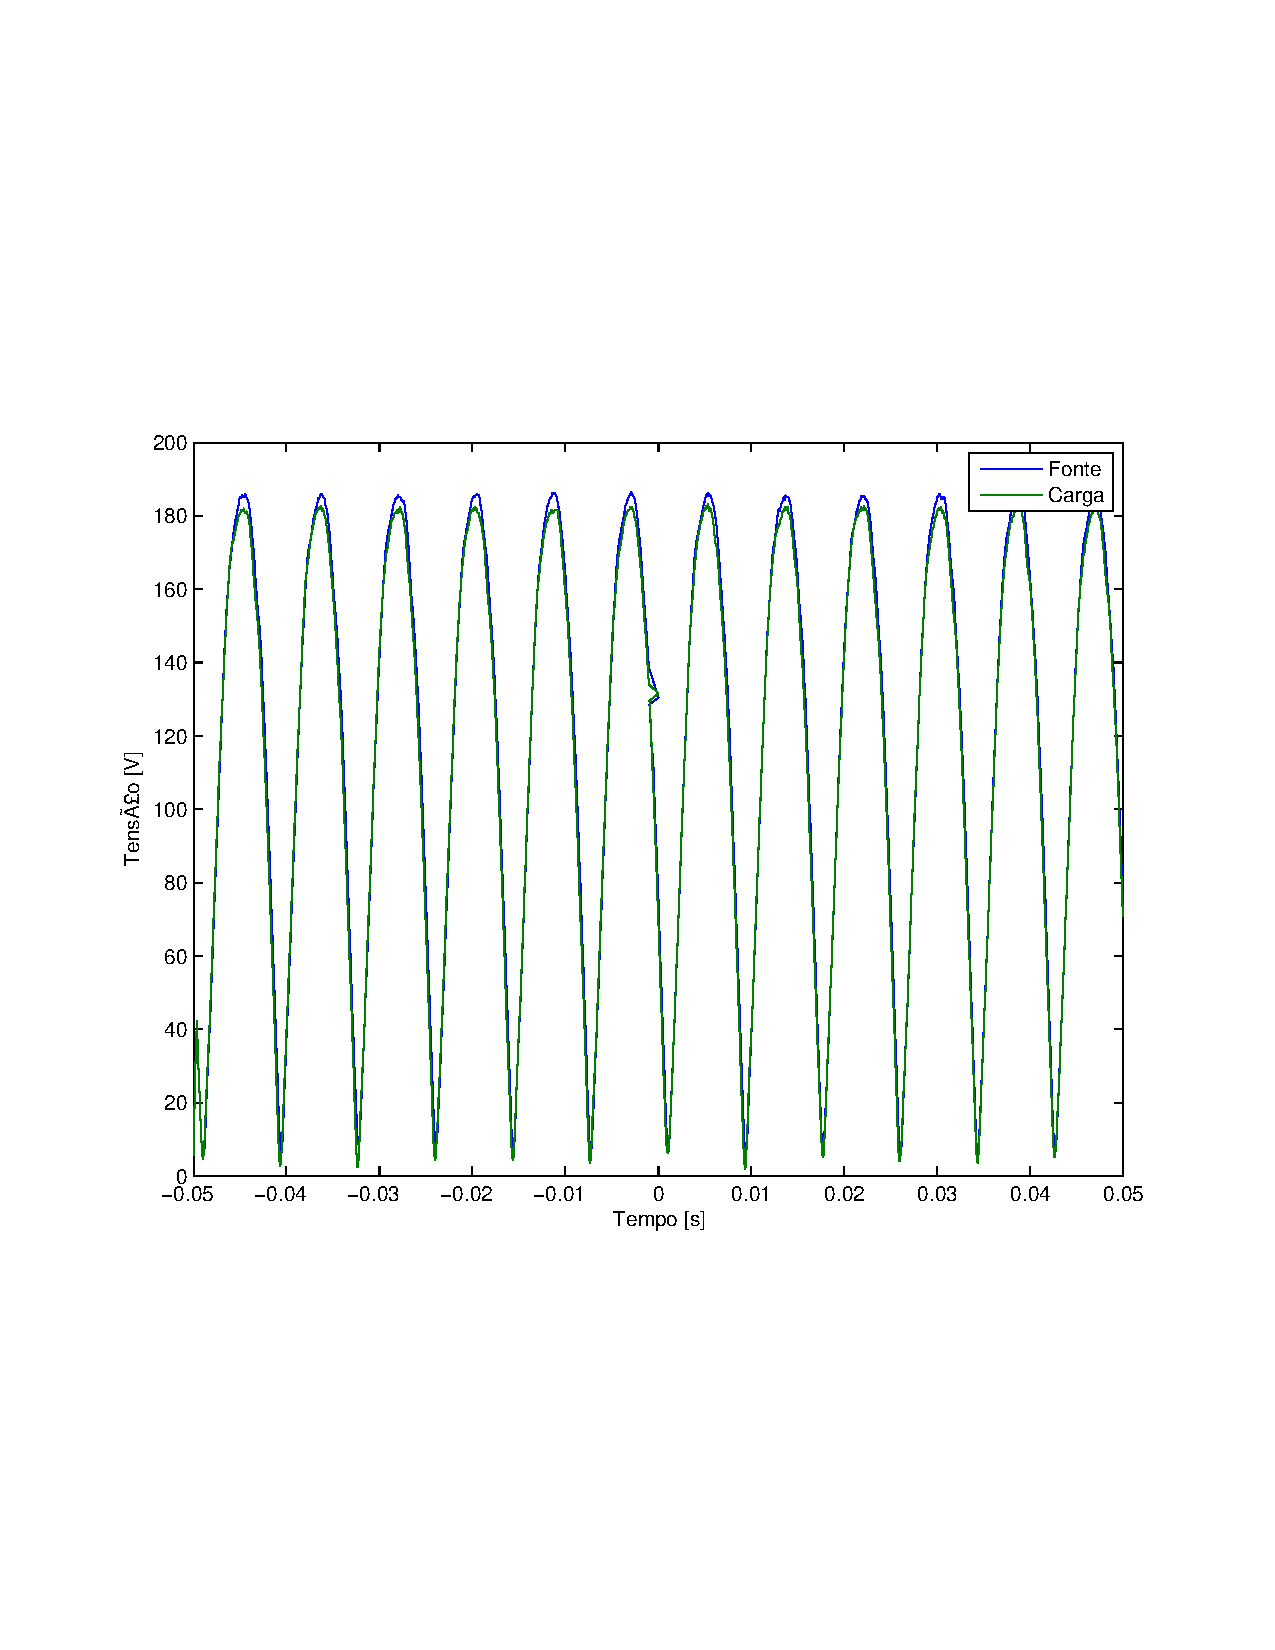
\includegraphics[width=\linewidth]{dados/monofasico/abs}
	\caption{Comparação entre valor absoluto da tensão na fonte e na carga}
	\label{fig:abs}
\end{figure}

\begin{figure}[H]
	\centering
	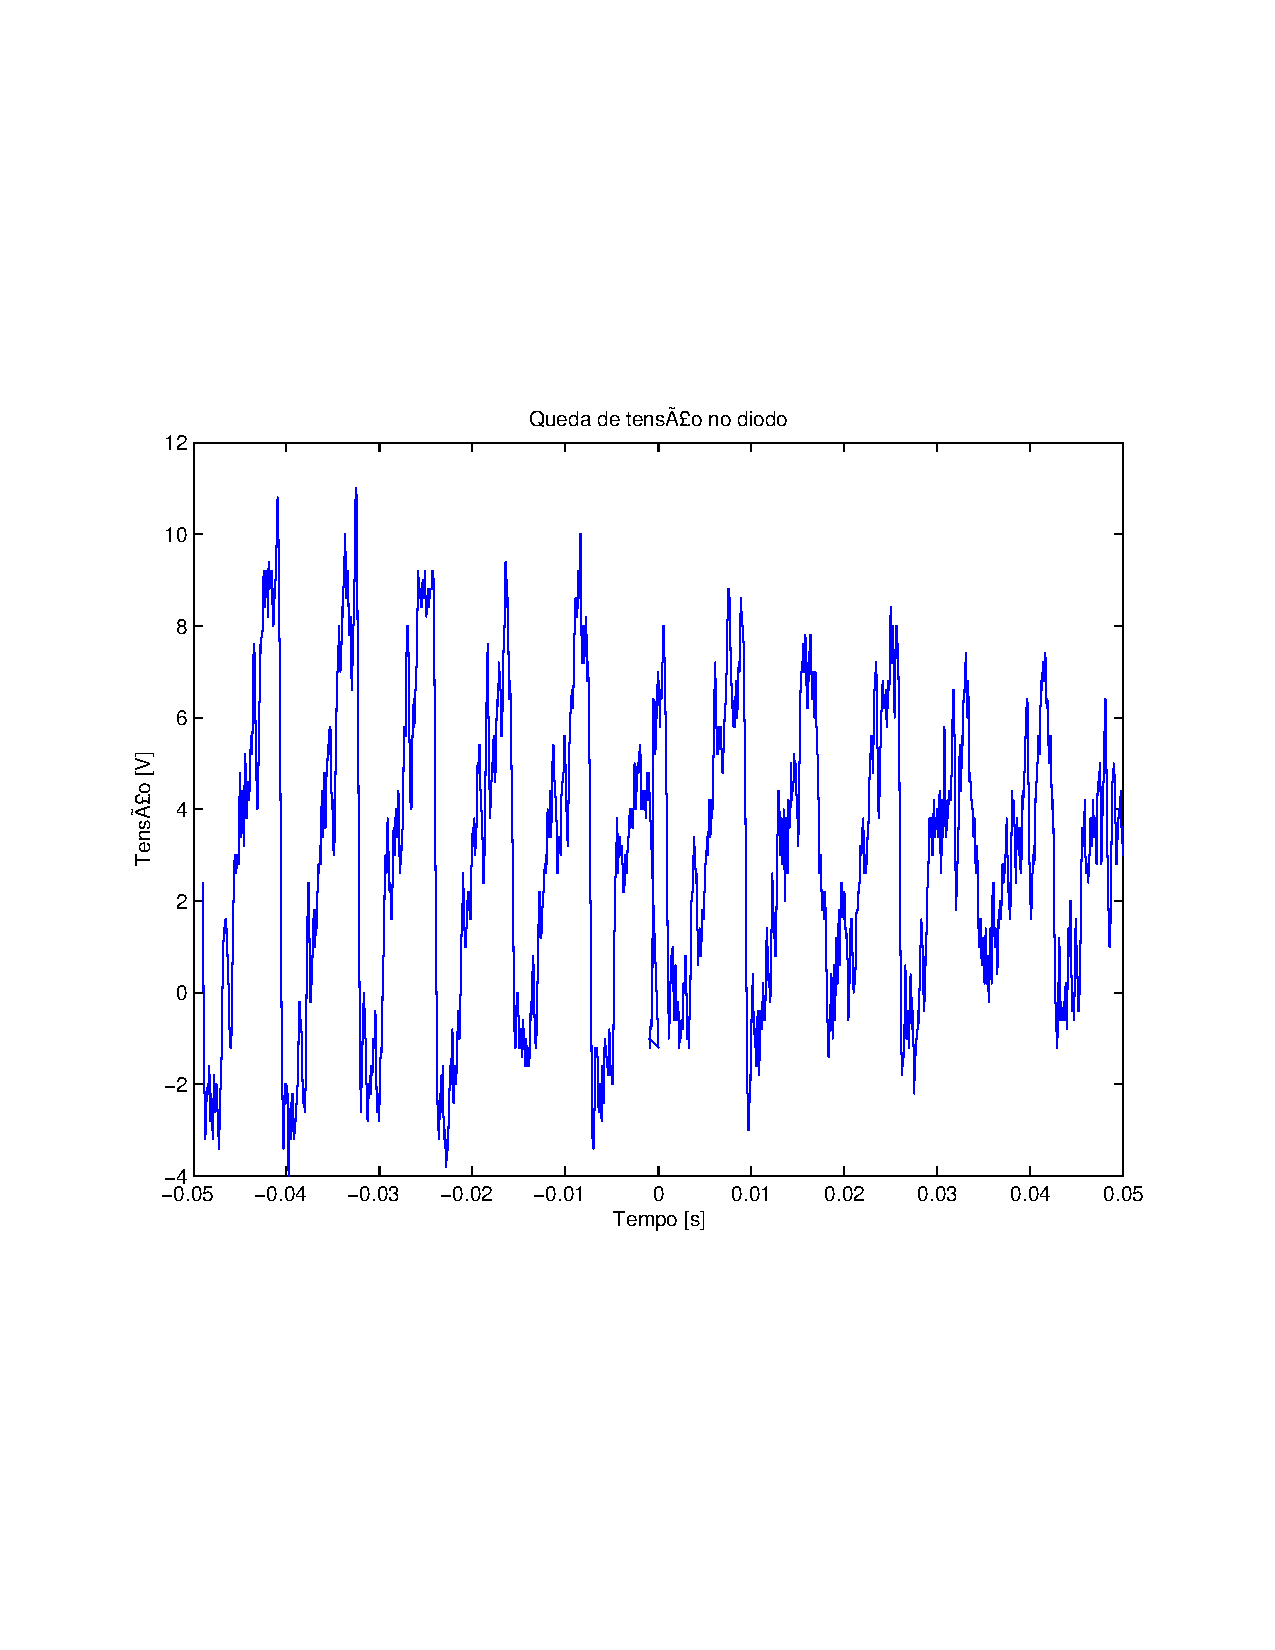
\includegraphics[width=\linewidth]{dados/monofasico/diff}
	\caption{Diferença entre valor absoluto da tensão na fonte e na carga}
	\label{fig:diff}
\end{figure}

Encontramos o valor médio dessa diferença, que foi de aproximadamente $2.954 V$, valor condizente com as diferenças entre os valores medidos e teóricos.

\section{Retificador trifásico}
De maneira semelhante ao monofásico, montamos o retificador de onda completa não controlado para fonte trifásica. Adicionando algumas ligações para as duas outras fases e rearranjando a ligação entre os diodos e carga, conseguimos montar o circuito recomendado. Nota-se que a ligação do neutro é utilizada somente para captura de dados no osciloscópio nesta etapa. O esquema elétrico do sistema é detalhado no roteiro.

Posicionamos os canais do osciloscópio para capturar dados da tensão de saída do conversor (tensão aplicada nas duas lâmpadas). Religando a chave, obtivemos a leitura apresentada na figura \ref{fig:tri_r}. 

\begin{figure}[H]
	\centering
	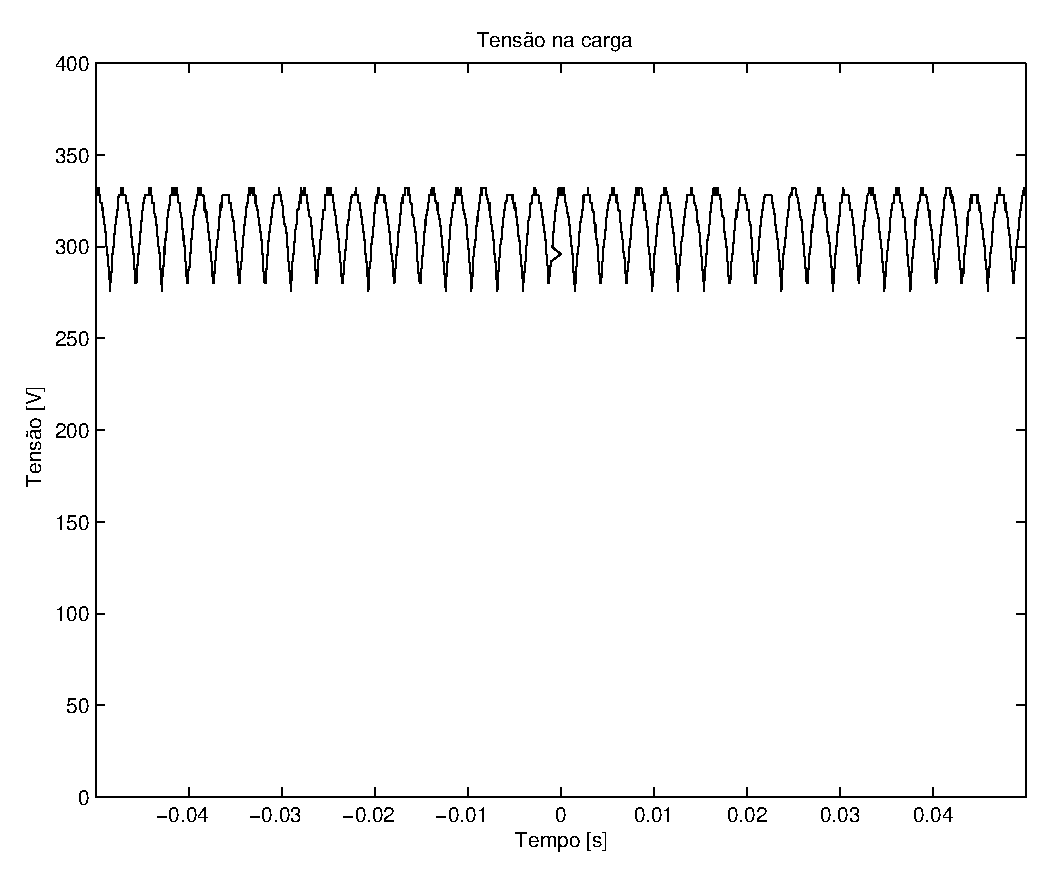
\includegraphics[width=\linewidth]{dados/trifasico/tri_r}
	\caption{Tensão medida na carga (duas lâmpadas em série)}
	\label{fig:tri_r}
\end{figure}

Ainda com auxílio do osciloscópio, verificamos os valores médio e RMS para a tensão na carga:
\begin{equation}
\overline{v_o} = 311\ V
\end{equation}
\begin{equation}
v_{o_{rms}} = 312\ V
\end{equation}

Notamos que a variação entre máximo e mínimo é bem menor quando comparada com o retificador monofásico, e que seu valor médio e rms são bem mais próximos do valor da tensão de linha, o que confirma que a capacidade de retificação é maior no trifásico que no monofásico.

Desligamos o circuito e reposicionamos as ponteiras do osciloscópio para calcular a tensão sobre a lâmpada 1, a mesma utilizada no ensaio do monofásico. Religamos o circuito e obtivemos os resultados apresentados na figura \ref{fig:tri_l1}.

\begin{figure}[H]
	\centering
	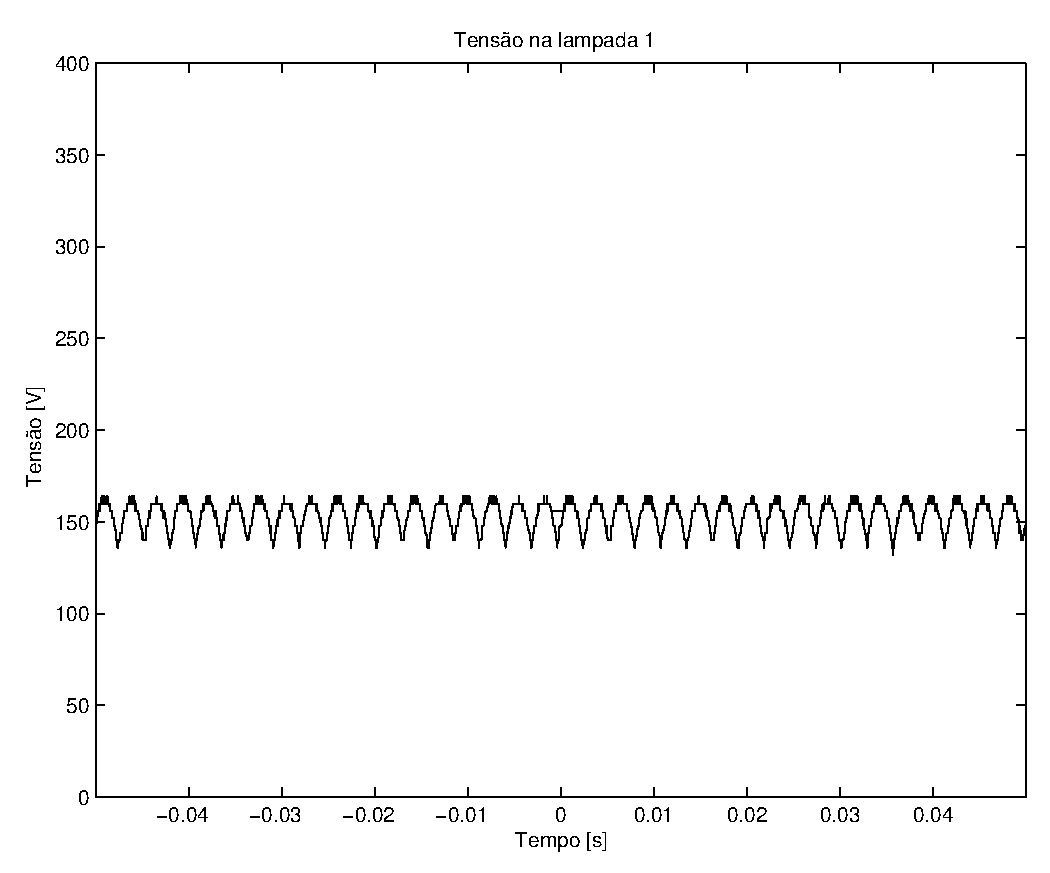
\includegraphics[width=\linewidth]{dados/trifasico/tri_l1}
	\caption{Tensão medida na lâmpada 1}
	\label{fig:tri_l1}
\end{figure}

Nesta lâmpada encontramos os valores médio e RMS a seguir:
\begin{equation}
\overline{v_L1} = 153\ V
\end{equation}
\begin{equation}
v_{L1_{rms}} = 153\ V
\end{equation}

Fizemos também a verificação de tensão no diodo $D1$ com o osciloscópio, obtendo a curva exibida na figura \ref{fig:tri_d1}. Notamos que durante o período de condução do diodo, sua tensão varia pouco quando comparada com a tensão do diodo do monofásico (figura \ref{fig:mono_d3}), mas a relação entre condução/corte é menor.

\begin{figure}[H]
	\centering
	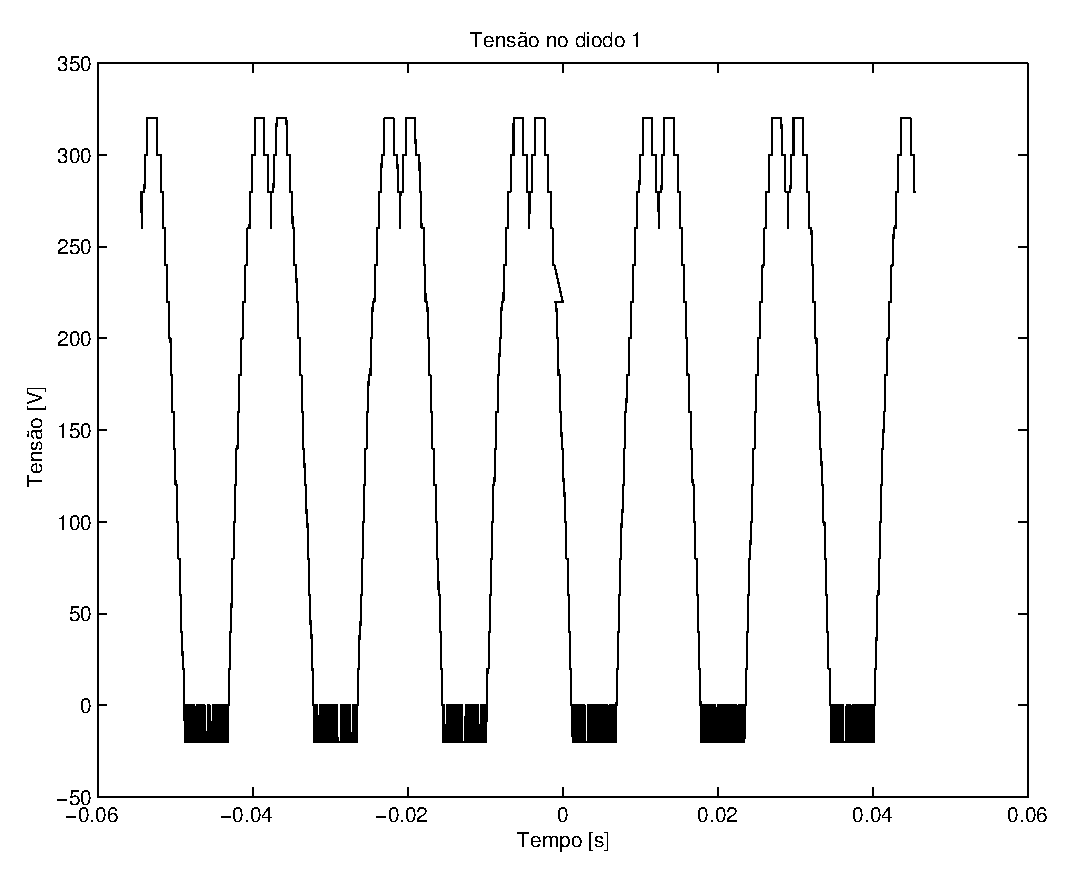
\includegraphics[width=\linewidth]{dados/trifasico/tri_d1}
	\caption{Tensão medida no diodo D1}
	\label{fig:tri_d1}
\end{figure}

Após o ensaio desligamos o circuito e medimos com auxílio do multímetro a resistência da segunda lâmpada, obtendo como resultado $R_2=56.9\ \Omega$.

Podemos calcular a tensão média teórica sobre a carga total através da equação \ref{eq:tmean}.
\begin{equation}
	\overline{V_o} = \frac{3}{\pi} \int_{\frac{\pi}{6}}^{\frac{4\pi}{6}}{Vs(sin(\theta) - sin(\theta - \frac{2\pi}{3}))d\theta} = \frac{3\sqrt{3}Vs}{\pi}
	\label{eq:tmean}
\end{equation}
Para calcular o valor efetivo da tensão sobre a carga utilizamos a equação \ref{eq:trms}.
\begin{equation}
	V_{o_{rms}} = \sqrt{\frac{3}{\pi} \int_{\frac{\pi}{6}}^{\frac{3\pi}{6}}{Vs^2(sin(\theta) - sin(\theta - \frac{2\pi}{3}))^2 d\theta}} = \sqrt{\frac{3}{2} + \frac{9\sqrt{3}}{4\pi}}Vs
	\label{eq:trms}
\end{equation}
Utilizando os valores da fonte ($Vs\ =\ \frac{330}{\sqrt{3}}\ V$), encontramos as tensões e correntes esperadas:
\begin{equation}
	\overline{V_o} = 315.12\ V
\end{equation}
\begin{equation}
	V_{o_{rms}} =  315.40\ V
\end{equation}
Conforme podemos ver os valores medidos e esperados diferem levemente, isso acontece devido a uma série de fatores, entre eles a queda de tensão nos diodos, as variações na tensão da fonte e as imprecisões da medida.
\bibliography{mybib}
\end{document}

